\documentclass[a4paper,10pt]{article}

\usepackage{polski}
\usepackage{moreverb}
\usepackage[latin2]{inputenc}
\usepackage{makeidx}
\usepackage{graphicx}

%============================= Definicje makr=============================
% finicja naglowka posrodku strony
\newcommand{\nagl}[1]{\par\begin{center}{\bf{#1}}\end{center}\par}
% Definicja tego na poczatku
\newcommand{\pocz}{\par {\bf{\nazwaprojektu}}\par {\bf{\nazwadokumentu}}\par {\bf{Wersja: \wersjadokumentu}}\par} 
%% Historia
% environment
\newenvironment{historia}{\nagl{Historia}\begin{tabular*}{17cm}{c|c|c|l} {\bf{Data}} & {\bf{Wersja}} & {\bf{Autor}} & {\bf{Zmiany}} \\}{\end{tabular*}}
% item
\newcommand{\hist}[4]{#1 & #2 & #3 & \parbox[t]{8cm}{#4} \\ }

% Marginesy
\textwidth17cm \textheight24.5cm \topmargin-40pt
\oddsidemargin-0.04cm
%=========================================================================

\makeindex 

	
\providecommand{\loxim}{LoXiM}
%\newcommand{\nazwaprojektu}{\loxim}

\newcommand{\nazwadokumentu}{Analiza mo�liwo�ci wykorzystania protoko�u LDAP
do obs�ugi dost�pu do semistrukturalnej BD} 

\newcommand{\wersjadokumentu}{0.1}

\title{\nazwadokumentu}
\author{Piotr Tabor (pt214569@students.mimuw.edu.pl)}


\begin{document}
\maketitle

\begin{historia}
	\hist{2008-03-09 -- 2008-03-26}{0.1}{Piotr Tabor}{Pierwsza wersja dokumentu}
	\hist{2008-03-09 -- 2008-06-03}{0.2}{Piotr Tabor}{Analiza i podsumowanie}
\end{historia}

\tableofcontents

\newpage


\providecommand{\LDAP}{Lightweight Directory Access Protocol wersja 3}
\providecommand{\loxim}{LoXiM}
\providecommand{\patrz}[1]{(patrz \ref{#1})}
\newcommand{\triple}[3]{$<$#1,#2,#3$>$}

\section{Wprowadzenie}

\subsection{Cel}
Celem tego  dokumentu jest przeanalizowanie mo�liwo�ci wykorzystania protoko�u
LDAP (\LDAP) jako podstawowego
narz�dzia do komunikacji z semistrukturaln� baz� danych z dost�pem za pomoc� 
j�zyka SBQL. 

W dokumencie zostan� tak�e przedstawione propozycje rozszerze� protoko�u, tak
by mo�na by�o za pomoc� protoko�u LDAP wraz z opisanymi rozszerzeniami wykorzysta�
pe�n� funkcjonalno�� systemu \loxim.

\subsection{Us�ugi katalogowe}

\subsection{Protok� LDAP a ,,Us�uga katalogowa LDAP'' (LDAP service)}
	Nale�y rozr�ni� dwa poj�cia:
	\begin{description}
		\item[Protok� LDAP] ---
			Jest to protok� komunikacyjny --- standard specyfikuj�cy zasady komunikacji
			pomi�dzy aplikacj� klienck�, a serwerem udost�pniaj�cym dane. Wnosi on tylko
			podstawowe za�o�enia o modelu danych.
		  
		\item[Us�uga katalogowa LDAP (LDAP (enabled) service)] --- 
			Jest to us�uga z kt�r�  mo�na si� komunikowa� przy pomocy protoko�u LDAP. 
			Realizuje ona wiele r�nych standard�w. W szczeg�lno�ci w sk�ad us�ugi
			katalogowej LDAP wchodzi obs�uga:
			\begin{itemize}
 				\item Modelu danych --- RFC4512 (Directory Information Models)
      			\item  Dost�pnych podstawowych metod autoryzacji --- RFC4513
      			(Authentication Methods and Security Mechanism)
      			\item Reprezentacji w postaci napis�w nazw znacz�cych (adres�w) -
      			RFC4514 (String Representation of Distinguished Names)
      			\item Reprezentacji zapyta� (filtr�w wyszukiwania) w postaci napis�w
      			- RFC4515 (String Representation of Search Filters)
      			\item Jednolitych wska�nik�w do zasob�w --- RFC4516 (Uniform Resource
      			Locator)
      			\item Zasad sk�adniowych i zasad dopasowywania danych --- RFC4517
      			(Syntaxes and Matching Rules)
      			\item Obs�ugi mi�dzynarodowych napis�w --- RFC4518 (Internationalized
      			String Preparation)
      			\item Schematu dla aplikacji u�ytkowych --- RFC4519 (Schema for User
      			Applications)
			\end{itemize} 
    \end{description}
		
	W poni�szym  dokumencie (o ile nie zaznaczono inaczej) pod terminem LDAP
	rozumiem ,,Protok� komunikacyjny LDAP''.
	
\subsection{Sposoby integracji serwera SBQL z us�ug� LDAP}

\label{wspolne}
Semistrukturalne bazy danych oraz us�ugi katalogowe ��czy wiele cech wsp�lnych.
W przypadku \loxim'a do najwa�niejszych z nich nale�y zaliczy�:
\begin{itemize}
  \item Obie us�ugi zajmuj� si� organizacj� i udost�pnianiem danych wed�ug
  zadanych przez u�ytkownika kryteri�w. 
  \item Obie us�ugi przechowuj� dane w strukturze drzewiastej.
  \item Obie us�ugi przewiduj� poj�cie odno�nika pomi�dzy w�z�ami tego drzewa.
  W przypadku LDAP jest to nazywane  ,,aliasem'', a w przypadku struktury SBQL
  obiektem wska�nikowym (ang. pointer object). 
  \item Obie us�ugi przewiduj� mo�liwo�� rozproszenia (przechowywania cz�ci
  drzewa) na r�nych serwerach --- jednocze�nie organizuj�c proces przeszukiwania
  w ten spos�b, �e mo�liwe jest otrzymanie pe�nego wyniku dla zapytania
  dotycz�cego wi�kszej ilo�ci �r�de� danych.
\end{itemize}

Metody przeszukiwania dla struktury LDAP posiadaj� nast�puj�ce cechy
\begin{itemize}
  \item[-] Wyszukuj� w danym poddrzewie te WPISY, kt�rych warto�ci atrybut�w
  ,,pasuj�'' do wskazanych warto�ci.
  \item[-] Posiadaj� bogate mechanizmy definiowania poj�cia ,,pasowania''
  (odporno�� na wielko�� znak�w, funkcje szyfruj�ce i por�wnuj�ce napisy
  zaszyfrowane).
  \item[-] Wynikiem zapytania jest zawsze wskazany zbi�r atrybut�w spo�r�d
  wszystkich odnalezionych w�z��w spe�niaj�cych wskazany warunek. 
  \item[-] Ca�kowity brak wsparcia dla przeszukiwa� ��cz�cych dane pochodz�ce
  z r�nych w�z��w.  
  \item[-] Ca�kowity brak mo�liwo�ci uzyskania danych zagregowanych. 
\end{itemize}
W zwi�zku z tym, �e mechanizm zapyta� LDAP jest stosunkowo prosty --- umo�liwia
on bardzo efektywn� realizacj� operacji (w pe�ni r�wnoleg�e i z wykorzystaniem niewielkiej
pami�ci pomocniczej przetwarzanie). Ogromn� wad� stanowi natomiast niewielka ilo�� operacji,
kt�r� z u�yciem tego narz�dzia mo�na przeprowadzi�.

W zastosowaniach rzeczywistych --- ograniczenie powy�sze prowadzi do
przechowywania cz�ci istotnych danych z us�ugi katalogowej w krotkach
relacyjnych bazy danych --- kt�re to umo�liwiaj� przeprowadzanie z��cze� danych
nale��cych do r�nych encji. W szczeg�lno�ci je�li mamy struktur� LDAP
przechowuj�c� dane osobowe pracownik�w, wykorzystywana do przeprowadzania
autoryzacji do oprogramowania korporacyjnego, to tak�e musimy mie� relacyjn�
kopi� tych danych na potrzeby dzia�ania oprogramowania finansowego lub
kadrowego.  Ubogo�� tych mechanizm�w prowadzi wi�c do redundancji, a tym samym 
do dodatkowych nak�ad�w na utrzymanie tych danych i brak generycznych
mechanizm�w zapewniaj�cych ich sp�jno��. 

Wydaje si�, �e sytuacja by�aby o wiele lepsza, gdyby jednocze�nie do danych 
obs�ugiwanych przez us�ug� katalogow� istnia� dost�p za pomoc� j�zyka zapyta�
o niepor�wnywalnie wi�kszych mo�liwo�ciach. Wtedy odpowiednia baza danych
umo�liwiaj�ca dost�p poprzez obydwa interfejsy mog�aby pe�ni� rol� centralnego
�r�d�a danych. 

Poni�ej przedstawiamy 3 og�lne schematy systemu realizuj�cego t�
funkcjonalno��.

\subsubsection{Serwer SBQL jako zaplecze (ang. backend) us�ugi LDAP}
	\begin{figure}[hbt]
		\centering
		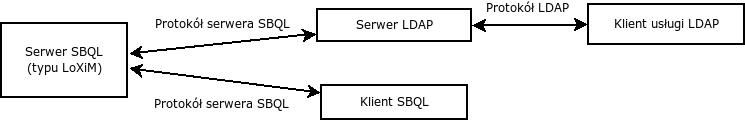
\includegraphics[scale=0.5]{img/ServerSBQLjakoBackendLDAP.jpg}
		\caption{Schemat serwera SBQL jako zaplecza us�ugi LDAP}
	\end{figure}  
	
W schemacie tym mamy zwyk�� baz� danych realizuj�c� dost�p poprzez j�zyk SBQL
oraz serwer LDAP wykorzystuj�cy t� baz� danych jako narz�dzie do przechowywania
i wyszukiwania informacji. Do serwera us�ugi LDAP jest zapewniony dost�p za
pomoc� protoko�u LDAP. Inne systemy chc�ce analizowa� dane przy pomocy SBQL'a
powinny dostawa� si� bezpo�rednio do bazy danych SBQL. 

Jest to najbardziej naturalne rozwi�zanie od strony implementacyjnej i
architektonicznej. Istniej� w nim dwa prawie niezale�ne komponenty skupione na
�wiadczeniu konkretnych us�ug. 

Zastosowanie tego modelu rodzi nast�puj�ce spostrze�enia:
\begin{itemize}
  \item Nie istnieje �adna zale�no�� pomi�dzy protoko�em dost�pu do bazy danych
  SBQL, a protoko�em LDAP. 
  \item Przechowywanie danych poprzez serwery us�ug katalogowych w
  semistrukturalnych, obiektowych bazach danych wydaje si� by� o wiele lepszym
  rozwi�zaniem ni� wykorzystywanie do tego celu relacyjnych baz danych (np.
  oprogramowanie OpenLDAP przechowuje dane w bazie Berkeley DB). Mo�na si�
  spodziewa�, �e z czasem powstan� narz�dzie zorganizowane w ten spos�b.
  \item Opracowanie jednego standardu przechowywania danych us�ug katalogowych
  w bazach typu \loxim{} --- zanim powstan� r�ne realizacje us�ug opartych na tym modelu --- 
  umo�liwi �atwiejsz� wymian� konkretnej implementacji us�ugi LDAP lub budowania
  wielu program�w korzystaj�cych z drzewa typu LDAP poprzez j�zyk SBQL. Dlatego
  w rozdziale ,,Symulowanie modelu danych protoko�u LDAP za pomoc� modelu
  danych SBQL'' (rozdzia� \ref{SymulowanieLDAPbySBQL}) spr�bujemy
  przeanalizowa� dost�pne mo�liwo�ci w tej kwestii.
  \item Istnieje ryzyko, �e modyfikacje danych przeprowadzane za pomoc� j�zyka
  SBQL b�d� narusza�y warunki stawiane strukturze danych serwera SBQL
  symuluj�cej katalog SBQL. Dlatego wskazane jest by taki schemat danych by�
  kontrolowalny pod wzgl�dem sp�jno�ci za pomoc� mechanizm�w serwera SBQL. 
\end{itemize}


\subsubsection{Serwer LDAP �wiadcz�cy dost�p za pomoc� j�zyka SBQL}
	\begin{figure}[hbt]
		\centering
		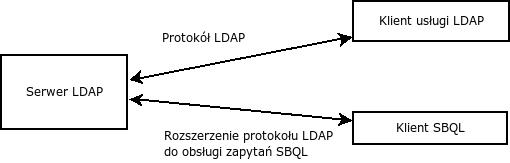
\includegraphics[scale=0.5]{img/ServerLDAPzDostepemSBQL.jpg}
		\caption{Schemat serwera LDAP z dost�pem przez SBQL}
	\end{figure}

Alternatywnym scenariuszem jest sytuacja, w kt�rej obecne rozwi�zania LDAP
zacz�yby by� rozszerzane do obs�ugi j�zyka typu SBQL. Wtedy naturalnym
rozwi�zaniem jest wprowadzenie do protoko�u LDAP rozszerzenia (nowych typ�w
pakiet�w), kt�re umo�liwi� zadawanie zapyta� w j�zyku SBQL, zamiast
implementowania na serwerze LDAP zupe�nie innego protoko�u. 

W realizacji tego rozwi�zania b�dzie potrzebny standard m�wi�cy 
jakiej strukturze danych serwera SBQL odpowiada dany katalog LDAP, a wi�c
opisuj�cy w jaki spos�b wykonywa� zapytania SBQL. Problem ten zosta� 
rozwini�ty w rozdziale \ref{SymulowanieLDAPbySBQL} ,,Symulowanie modelu danych
protoko�u LDAP za pomoc� modelu danych SBQL''. 

Drugim brakuj�cym elementem jest specyfikacja rozszerzenia protoko�u LDAP,
umo�liwiaj�ca w tym protokole wykonywanie zapyta� SBQL. Problemem tym zajmujemy
si� w rozdziale \ref{RozszerzenieLDAP}. 

\subsubsection{Serwer SBQL �wiadcz�cy dost�p do danych za pomoc� protoko�u LDAP}
\begin{figure}[hbt]
	\centering
	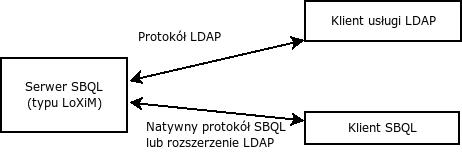
\includegraphics[scale=0.5]{img/ServerSBQLzDostepemLDAP.jpg}
	\caption{Schemat serwera SBQL �wiadcz�cego dost�p do danych za pomoc�
	protoko�u LDAP}
\end{figure}  

W tym modelu rozpatrujemy serwer SBQL, kt�ry nie tylko obs�uguje dost�p za
pomoc� j�zyka SBQL, ale tak�e udost�pnia zasoby za pomoc� mechanizm�w protoko�u
LDAP. Gdyby mo�liwe by�o sensowne wykonywanie wyszukiwa� LDAP oraz polece�
modyfikuj�cych dane protoko�u LDAP na ka�dym modelu danych serwera SBQL (modelu
$AS_0$ lub wy�szego) to realizacja tego modelu mia�a by sens. Umo�liwi�aby ona
wykorzystanie ju� istniej�cych rozwi�za� integruj�cych si� z us�ugami
katalogowymi i operowanie bezpo�rednio na bazie typu \loxim.

Kwestiami wykonywania operacji protoko�u LDAP na og�lnym modelu danych
serwera SBQL ($AS_0$) zajmiemy si� szczeg�owo w rozdziale \ref{OperacjeLDAPw$AS_0$}.

By nie mno�y� byt�w w tym rozwi�zaniu mia�oby sens zastosowanie
jednego protoko�u dost�pu --- kt�rym by�by protok� LDAP wraz z pewnymi
rozszerzeniami umo�liwiaj�cymi wykorzystywanie j�zyka SBQL do przeprowadzania
zapyta�. S� to te same rozszerzenia, kt�re dotycz� ,,Serwera LDAP �wiadcz�cego
dost�p za pomoc� j�zyka SBQL'' i kt�re szczeg�owo omawiamy w rozdziale
\ref{RozszerzenieLDAP}. 
		
\section{Analiza}

\subsection{Por�wnanie modeli danych}

\subsubsection{SBQL}

Rozwa�my najbardziej og�lny model danych dla j�zyka
SBQL --- ($AS_0$ Store Model). W modelu tym obiekty s� 
tr�jkami \triple{identyfikator}{nazwa}{warto��}, w kt�rych wyr�niamy
w trzy przypadki:
\begin{description}
	\item[Obiekty atomowe (proste)] --- (ang. atomic objects)
	\triple{identyfikator}{nazwa}{warto�� prosta}
	\item[Obiekty wska�nikowe] --- (ang. pointer objects)
	\triple{identyfikator}{nazwa}{identyfikator docelowy}
	\item[Obiekty z�o�one] --- (ang. complex objects)
	\triple{identyfikator}{nazwa}{kolekcja obiekt�w}
	Gdzie kolekcja obiekt�w mo�e by� zbiorem (ang. set) b�d�
	sekwencj� (ang. sequence) element�w (w modelu $AS_{0_{seq}}$)
\end{description} 

Model ten narzuca dodatkowo pewne wymagania dotycz�ce ``zgodno�ci'' danych:
\begin{itemize}
	\item Unikatowo�� identyfikator�w obiektu. W ca�ym systemie nie istniej� 
	dwa elementy o takim samym identyfikatorze (pierwszym elemencie tr�jki)
	\item Je�eli obiekt jest typu wska�nikowego, to obiekt na kt�ry wskazuje musi
	istnie�
\end{itemize} 

Dodatkowo obowi�zuje za�o�enie ca�kowicie ukrytego identyfikatora (Total
internal object identification) w ,,Principles of query programming languages'' \cite{SBQL},
kt�re oznacza, �e u�ytkownik (aplikacja kliencka) nie mo�e pozna� identyfikatora
obiektu z kt�rym pracuje. Zatem w tym modelu danych nie istnieje �aden
zewn�trzny identyfikator (adres), kt�ry by potrafi� unikatowo zidentyfikowa�
konkretny obiekt w ca�ej bazie danych implementuj�cej ten model.  

\subsubsection{Model danych LDAP}
	Dane s� reprezentowane w postaci hierarchii obiekt�w (wpis�w) (ang. entries).
	Szczytowe (ang. top) obiekty takiego drzewa nazywane s� korzeniami (ang.
	roots/base/suffixs). Ka�dy obiekt ma maksymalnie jednego ojca i mo�e mie� dowoln� liczb�
	dzieci oraz zbi�r atrybut�w. 
	
	Ka�dy atrybut ma nazw� i mo�e mie�  jedn� lub
	wiele warto�ci. Warto�ci w obr�bie pojedynczego atrybutu nie mog� by� to�same
	 (definicja to�samo�ci zale�y od atrybutu (matching rule). Kolejno�� warto�ci w
	 obr�bie atrybutu o wielu warto�ciach nie ma znaczenia. 
	 Mo�na my�le� o atrybucie z wieloma warto�ciami jak o wielu atrybutach z tak� 
	sam� nazw� i r�nymi warto�ciami. 
	
	Dla r�nych atrybut�w mo�e by� w r�nych spos�b zdefiniowana identyczno��
	(matching rule). W szczeg�lno�ci specyfikacja, czy por�wnanie jest zale�ne
	od wielko�ci znak�w (case sensitive/insensitive) jest najcz�ciej u�ywan�
	w�asno�ci� atrybutu. 
	
	Obiekty od danego korzenia buduj� drzewo DIT (Directory Information Tree). W
	obr�bie drzewa ka�dy obiekt mo�na zaadresowa� za pomoc� DN (Distinguish
	Name). DN buduje si� jako ci�g obiekt�w par: (atrybut=warto��), specyfikuj�cych 
	pe�n� �cie�k� od obiektu do korzenia.
	
	Np. cn=Piotr Tabor,ou=MIMUW,o=UW,city=Warszawa,country=Polska.
	
	Protok� LDAP przewiduje istnienie alias�w, kt�re polegaj� na tym, �e 
	element mo�e pokazywa� na Distinguish Name innego elementu. Z punktu widzenia
	przeszukiwania (o ile flaga dereferencji alias�w w zapytaniu jest w��czona)
	taki element jest traktowany jakby nale�a� do poddrzewa. Linki te mo�na
	rozumie� jako analogi� do dowi�za� symbolicznych w systemach Uniksowych.
	
	
	\begin{figure}[hbt]
		\centering
		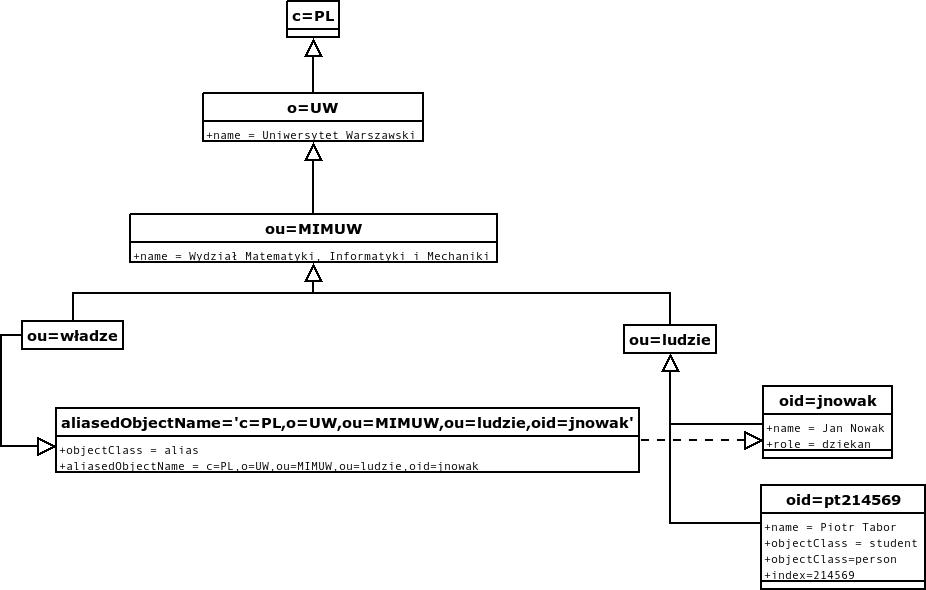
\includegraphics[scale=0.5]{img/ldap_mimuw.jpg}
		\caption{Przek�ad 1 danych w modelu LDAP}
	\end{figure}  

% \subsection{Por�wnanie cech obu modeli}
% 
% \begin{tabular*}{17cm}{|l|l|l|}
% 	\hline
% 	\bf{Cecha} & \bf{LDAP} & bf{$AS_0$ (SBQL)} \\
% 	\hline
% 	
% 	Jednostki danych & Atrybuty, dzieci &  Uto�samione zosta�y atrybuty i
% 	podobiekty (dzieci)\\
% 	
% 	Identyfikacja	 & 
% 	
% 	Aliasy 			 &	
% \end{tabular*} 

	
\subsection{Symulowanie modelu danych protoko�u LDAP za pomoc� modelu
danych SBQL}
\label{SymulowanieLDAPbySBQL}
\subsubsection{Podej�cie 1}

Na podstawie danych w modelu LDAP mo�na zbudowa� ich instancj� w modelu $AS_0$
w nast�puj�cy rekurencyjny spos�b (za��my, �e mamy zbudowa� struktur� dla
poddrzewa zaczynaj�cego si� w danym wpisie E):

Tworzymy obiekt okalaj�cy o id ($i_1$), zawieraj�ce nast�puj�cy wi�zania
 (bindings):
 	\begin{description}
 		\item[entry] --- obiekt (wpis) w�a�ciwy.
 			\begin{itemize}
 				\item Dla ka�dego atrybutu nale��cego do wpisu E tworzymy wi�zanie o nazwie
 				atrybutu prowadz�ce do warto�ci tego atrybutu.
 			
 				\item  Dla atrybutu kluczowego (buduj�cego 	,,distinguish name'') tworzymy
 				wi�zanie o nazwie atrybutu poprzedzonej '\#' prowadz�ce do warto�ci
 				atrybutu kluczowego.
 				
 				\item Dla ka�dego wpisu bezpo�rednio podleg�ego tworzymy binding o nazwie
 				'\#child\#' prowadz�cy do rekurencyjnie wygenerowanego dla
 				tego wpisu obiektu okalaj�cego. 
			\end{itemize}
 		\item[deref] -
 			Je�eli bie��cy wpis jest aliasem to ,,deref'' wskazuje na cel aliasu
 			(bezpo�rednio, a nie na obiekt okalaj�cy). W przeciwnym przypadku wi��e do
 			tego samego obiektu co ,,entry''.
	\end{description}


Przyk�ad z rysunku przedstawionym w ``Modelu danych LDAP'', zapisany w $AS_0$ z
wykorzystaniem tego podej�cia (po dodaniu nadrz�dnych obiekt�w root i
\#child\#): \begin{verbatimtab}[3] 1 root:
	2 #child#:
		3 deref: ->5
		5 entry:
			6 c=PL
			7 #c -> 6
			8 #child#:
				9 deref: ->10
				10 entry:
					11 ou=UW
					12 #ou -> 11
					13 name=Uniwersystet Warszawski
					14 #child#:
						15 deref: ->16
						16 entry: 
							17 ou=MIMUW
							18 #ou=MIMUW
							19 name=Wydzia� Matematyki, Informatyki i Mechaniki
							20 #child#
								21 defer: ->22
								22 entry: 
									23 ou=ludzie
									24 #ou ->23
									25 #child#
										26 deref ->27
										27 entry:
											28: oid=jnowak
											29: #oid ->28
											30: name=Jan Nowak
											31: objectClass: person
											50: role: dziekan
									32 #child#
										33 deref ->34
										34 entry:
											35: oid=pt214569
											36: #oid ->35
											37: name=Piotr Tabor
											38: index=214569
											39: objectClass: person
											40: objectClass: student
							41 #child#
								42 deref: ->43
								43 entry: 
									44 ou=W�adze
									45 #ou ->44 
									46 #child#:
										47 deref ->27
										48 entry:
											49 aliasedObjectName='c=PL,o=UW,ou=MIMUW,ou=ludzie,oid=jnowak'	
											51 #aliasedObjectName ->49
											52 objectClass: alias										
\end{verbatimtab}

W tym modelu mo�emy stosunkowo �atwo przet�umaczy� ,,distinguish name'' na
zapytanie odnajduj�ce wskazany adres.
Nast�puj�cy adres: c=PL,o=UW,ou=MIMUW,ou=ludzie,oid=jnowak zostanie
przet�umaczony na:
\begin{description}
	\item[W przypadku nie rozwijania alias�w]:\\
	(root).(entry where \#c=PL).\#child\#.(entry where \#ou=UW).\#child\#\\
	.(entry	where \#ou=MIMUW).\#child\#.(entry where \#ou=ludzie).\#child\#\\
	.(entry where \#oid=pt214569).\#child\#
	\item[W przypadku rozwijania alias�w]:\\
	(root).(deref where \#c=PL).\#child\#.(deref where \#ou=UW) .\#child\#\\
	.(deref	where \#ou=MIMUW).\#child\#.(deref where \#ou=ludzie).\#child\#\\
	.(deref where \#oid=pt214569).\#child\# 
\end{description}

% \subsubsection{Podej�cie 2}
% 
% Wydaje si� istotnym post�pem, gdyby uda�o si� z podej�cia pierwszego usun��
% obiekty okalaj�ce. Tak naprawd� jedynym powodem, dla kt�rego je wprowadzili�my
% by�a konieczno�� rozr�niania przej�cia po wi�zaniu zwyk�ym
% (typu \triple{$i_1$}{name}{[zbi�r obiekt�w]}), a wi�zaniu typu wska�nik/link 
% (typu \triple{$i_1$}{name}{$i_2$}). Gdyby j�zyk SBQL wprowadzi� operator
% algebraiczny $is_pointer(i)$


\subsection{Operacje protoko�u LDAP} \label{OperacjeLDAPw$AS_0$}
	\subsubsection{Operacje protoko�u StartTLS}

		Wys�anie paczki StartTLS przez klienta protoko�u LDAP powoduje rozpocz�cie negocjacji TLS (Transport Layer Security), czyli
		bezpiecznego --- szyfrowanego --- po��czenia. Operacja ta jest istotna i w oczywisty spos�b �atwa do zaimplementowania
		w przypadku wykorzystania protoko�u do komunikacji z innym rodzajem bazy danych. 
	
	\subsubsection{Bind --- autoryzacja}

W protokole LDAP klient przeprowadzaj�c autoryzacj� przekazuje nast�puj�ce parametry serwerowi:
\begin{description}
	\item[wersje protoko�u] --- po kt�rej chce si� komunikowa� (obecnie dozwolona tylko wersja 3)
	\item[nazwa (DN) loguj�cego si�] --- adres (DN) wpisu identyfikuj�cego obiekt autoryzuj�cy si� (przewa�nie u�ytkownika)
	\item[dane autentykuj�ce] --- paczka danych opisuj�cych wybran� metod� autentykacji oraz zestaw danych potrzebnych do jej przeprowadzenia.
	Specyfikacja podstawowych metod znajduje si� w dokumencie \cite{RFC4520} i przewiduje: logowanie anonimowe, logowanie z podaniem loginu i has�a
	(czystego b�d� zaszyfrowanego) oraz us�ugi SASL (Simple Authentication and Security Layer). 
\end{description}   

Wykorzystanie tej metody w modelu bazy semistrukturalnej niesie ze sob� nast�puj�ce trudno�ci:
\begin{itemize}
  \item Zak�ada, �e u�ytkownicy bazy danych s� dost�pni jako element struktury danych. To za�o�enie wydaje
  si� sensowne. W najgorszym przypadku u�ytkownicy mog� by� udost�pniani jako fragment wirtualnego modelu danych (analogia do
  katalogu /proc w UNIX'ach).
  \item Zak�ada, �e dysponujemy mechanizmem t�umaczenia adres�w DN na konkretne obiekty modelu $AS_0$ (\patrz{SymulowanieLDAPbySBQL}) (w og�lnym przypadku danych -
  niemo�liwe lub bardzo si�owe)
\end{itemize}

Drugie z wymieniony za�o�e� jest problemem trudnym, ale przyjmuj�c nawet, �e jest nierozwi�zywalny z niewielk� strat� 
mo�emy przyj��, �e operacja BIND z atrybutem name=``o=loxim,cn=kowalski'' odpowiada pr�bie autentykacji u�ytkownika Kowalski do bazy danych. 

Reasumuj�c --- pakiet ten jest istotny i mo�liwe jest jego wykorzystanie przy dost�pie do bazy danych typu \loxim.  

\subsubsection{Unbind --- zako�czenie po��czenia}
Nazwa tego polecenia jest myl�ca, gdy� w protokole LDAP oznacza ona operacje zamkni�cia po��czenia 
(a nie --- jak mog�a by sugerowa� --- wylogowania u�ytkownika). 

Operacja nie niesie ze sob� �adnych trudno�ci w dost�pie do danych o semistrukturalnym modelu. 

\subsubsection{Search --- wyszukiwanie}
Operacja ,,search'' jest najwa�niejsz� operacj� w us�ugach katalogowych. Przyjmuje nast�puj�ce parametry: 
\begin{description}
	\item[baseObject] --- adres (DN) miejsca w drzewie od kt�rego (w g��b) rozpoczynamy przeszukiwanie
	\item[scope]      --- zakres drzewa, kt�ry chcemy przeszuka�:
		\begin{description}
			\item[baseObject] --- przeszukany zostaje tylko wskazany obiekt (w praktyce oznacza to sprawdzenie, czy wskazany obiekt spe�nia zadane warunki lub pobranie
			wybranych atrybut�w z obiektu)
			\item[singleLevel] --- przeszukane zostaj� (bezpo�rednie) dzieci danego obiektu
			\item[wholeSubtree] --- przeszukane zostaje ca�e poddrzewo wyznaczone przez ,,baseObject'', czyli wszyscy potomkowie tego obiektu z nim w��cznie  
		\end{description}
	\item[derefAliases] --- jak aliasy (odpowiednik obiekt�w pointerowych) maj� by� traktowane:
		\begin{description}
			\item[neverDerefAliases]   --- nigdy nie interpretuj alias�w 
			\item[derefInSearching]    --- interpretuj aliasy tylko w trakcie przeszukiwania (ale nie w trakcie znajdowania ,,korzenia przeszukiwania'' (baseObject))
			\item[derefFindingBaseObj] --- interpretuj aliasy w trakcie znajdowania ,,korzenia przeszukiwania'' (baseObject)
			\item[derefAlways]         --- zawsze interpretuj aliasy
		\end{description}
	\item[sizeLimit] --- maksymalna liczba zwr�conych wpis�w
	\item[timeLimit] --- maksymalny czas przeszukiwania (w sekundach). W przypadku przekroczenia --- zwr�cone zostan� wpisy znalezione do czasu jego up�yni�cia. 
	\item[typesOnly] --- true lub false --- decyduje, czy zapytanie zwraca pary: opis atrybutu i jego warto��, czy tylko opisy atrybut�w 
	\item[filters] --- z�o�ony obiekt reprezentuj�cy warunki jakie musz� spe�nia� zwr�cone wpisy (obejmuje: por�wnania atrybut�w ze sta�ymi (tak�e przybli�one),
	operacje logiczne, sprawdzanie istnienia atrybutu). 
	\item[attributes] --- lista atrybut�w, kt�re maj� zosta� zwr�cone dla ka�dego znalezionego wpisu. Mo�na te� przekaza� warto�� ��daj�c� wszystkich atrybut�w
	zawartych w danym wpisie (bez ukrytych). 
\end{description} 

W odpowiedzi na t� operacj� b�d� przychodzi� (asynchronicznie): lista znalezionych obiekt�w z warto�ciami wskazanych atrybut�w --- a tak�e 
lista serwer�w, kt�re mog� zna� wi�cej odpowiedzi na to zapytanie (mo�e by� warto przeprowadzi� to samo przeszukiwanie
na nich, ale to decyzja klienta). 

Wykorzystanie tego mechanizmu do przeszukiwania bazy danych opartej na j�zyku SBQL wymaga:
\begin{itemize}
  \item przet�umaczenia adresu ,,baseObject'' na konkretny obiekt modelu $AS_0$ (czyli na zapytanie SBQL znajduj�ce ten obiekt) (\patrz{SymulowanieLDAPbySBQL}) z
  interpretacj� (lub nie) alias�w --- w zale�no�ci od warto�ci parametru ,,derefAliases'' (w og�lnym przypadku danych --- niemo�liwe lub bardzo si�owe) 
  \item  Przet�umaczenie warunk�w wyszukiwania zadanych parametrem ,,filter'' na SBQL'a --- uwzgl�dniaj�cego wybrany ,,scope'', a tak�e rozwijanie alias�w
  (,,deref aliases''). Zak�adaj�c, �e mo�emy sk�adnie SBQL'a rozszerzy� o funkcje dokonuj�ce bardziej z�o�onych por�wna� (np. z uwzgl�dnieniem skr�t�w MD5 lub
  SHA1) co wydaje si� w pe�ni realizowalne --- o ile wiemy jak interpretowa� poj�cie ,,wpis'' i ,,atrybut'' w kontek�cie przetwarzanych danych ($AS_0$). 
\end{itemize}

Problemy te --- je�li zak�adamy, �e baza danych zawiera dane w og�lnym modelu $AS_0$ wydaj� si� uniemo�liwia� przeprowadzenie tej operacji. Jednak na danych, kt�re
potrafimy zinterpretowa� jako ,,wpisy'' i ,,atrybuty'' mo�emy z powodzeniem i wydajnie zaimplementowa� t� operacj�. 

Operacja ta nie nadaje si� do zadawania zapyta� w j�zyku SBQL w szczeg�lno�ci ze wzgl�du na stosunkowo ,,p�aski'' format odpowiedzi, a tak�e  braku 
parametru umo�liwiaj�cego wygodne przekazanie zapytania SBQL wraz z warto�ciami jego parametr�w. Z tego wzgl�du --- je�li chcemy zapewni� mo�liwo�� zadawania
zapyta� SBQL bazie danych --- musimy zaimplementowa� now� operacj� do tego przeznaczon� (rozszerzenie protoko�u LDAP).  

\subsubsection{Modify --- zmiana wpisu}
Operacja ,,modify'' umo�liwia klientowi dodanie lub usuni�cie atrybut�w z wpisu, a tak�e zamian� warto�ci wskazanych atrybut�w. 
Zawiera dwa parametry:
\begin{description}
	\item[object] --- adres (DN) wpisu, kt�ry chcemy zmodyfikowa�. 
	\item[changes] --- list� operacji modyfikacji.
	Operacjami modyfikacji mo�e by�:
		\begin{description}
			\item[add]  --- dodanie atrybutu (lub warto�ci do atrybutu --- je�li ten ju� istnieje)
			\item[delete] --- usuni�cie ca�ego atrybutu (lub pojedynczej warto�ci --- je�li zosta�a ona wskazana) 
			\item[replace] --- zamienienie wszystkich warto�ci wskazanego atrybuty na za��czone do tej operacji. 
		\end{description}
\end{description} 

Przeprowadzenie tej operacji w bazie typu SBQL jest mo�liwe w sytuacji kiedy umiemy mapowa� poj�cia ,,wpis'' i ,,atrybut'' na model danych.
W og�lnym przypadku musimy odnale�� ,,object'' (czyli przet�umaczy� DN na zapytanie SBQL), a nast�pnie w zale�no�ci od wybranej operacji 
musieliby�my usun��, zmodyfikowa� lub doda� nowe dziecko typu ,,binder'' do wskazanego obiektu. Tworzony binder b�dzie zwi�zany z warto�ci� typu
prostego. 

\subsubsection{Add --- dodanie wpisu}

Operacja przyjmuje dwa parametry: adres (DN) wpisu, kt�ry chcemy utworzy� oraz list� atrybut�w wraz z warto�ciami dla tego obiektu.

Przy za�o�eniu, �e umiemy przet�umaczy� DN na obiekt modelu $AS_0$, kt�ry chcemy utworzy� --- operacj� t� 
mo�emy wykona� przez utworzenie prostego obiektu typu ,,binder'' dla ka�dego atrybutu we wskazanym obiekcie.  

\subsubsection{Delete --- usuni�cie wpisu}

Operacja usuwa wskazany wpis. Jej jedynym parametrem jest DN wpisu, kt�ry chcemy usun��. 

Przy za�o�eniu, �e umiemy przet�umaczy� DN na obiekt modelu $AS_0$, kt�ry chcemy usun�� --- ta operacja jest wykonywalna i istotna.  


\subsubsection{Abandon --- przerwanie przetwarzanej w�a�nie operacji}

Operacja ta przyjmuje parametr b�d�cy id wykonywanej aktualnie operacji (przewa�nie polecenia SEARCH) i wymusza jej zako�czenie. 

Operacja istotna i mo�liwa do implementacji w bazie danych opartej na SBQL.  

%\subsubsection{Symulowanie operacji protoko�u LDAP na bazie danych w modelu $AS_0$}
%\label{OperacjeLDAPw$AS_0$}

% \subsection{Zgodno��}
% 	Mo�liwe jest, by system \loxim{} realizowa� wszystkie powy�sze operacje, a tym
% 	samym by� ``pe�nym'' serwerem us�ugi katalogowej w rozumieniu protoko�u LDAP.
% 	
% 	Operacj� search, modify, delete i add bez wi�kszych problem�w mo�na
% 	przet�umaczy� na j�zyk SBQL. Jedynym wymaganiem jest, by SBQL
% 	implementowa� nast�puj�ce funkcje:
% 	\begin{description}
% 		\item[approxMatch] (RFC4511 (4.5.1.7.5)) --- zwracaj�c�,  czy dwa dane elementy
% 			,,prawie'' (np. fonetycznie, leksykalnie) do siebie pasuj�. Mo�na te� u�y�
% 			operacji ,,r�wna si�'' do najprostszej implementacji tej funkcji (t�umacz
% 			LDAP $\to$ SBQL przet�umaczy j� jako ,,r�wna si�``)
%     \end{description}
% 	
% 	Szczeg�lnie interesuj�ce wydaje si� po��czenie mo�liwo�ci relacyjnych baz
% 	danych (transakcje, skomplikowane regu�y wyszukiwania i aktualizacji danych) i
% 	us�ug katalogowych w jednym narz�dziu.
	

\subsection{Podsumowanie}

Pomimo wielu cech wsp�lnych obu narz�dzi \patrz{wspolne} wykorzystanie
czystego protoko�u LDAP jako jedynego interfejsu komunikacyjnego jest problematyczne.

Wykazali�my, �e operacje ,,bind'', ,,unbind'', ,,startTLS'', ,,abandon'' mo�na stosunkowo 
�atwo wykorzysta� w bazie danych typu SBQL (mo�na je wykorzysta� w ka�dym protokole, kt�ry
przeprowadza autentykacje). Stanowi� one ,,standardowy'' szkielet, na kt�rym mo�na budowa� 
protok� w�a�ciwy. 

Operacje ,,add'', ,delete'' i ,,modify'' jeste�my w stanie przeprowadzi� w bazie danych typu \loxim{} o ile 
potrafimy zinterpretowa� DN jako adres konkretnego obiektu w tej bazie. W praktyce jest to tylko mo�liwe je�li
baza u�ywa schematu, kt�ry jeste�my wstanie zinterpretowa� jako zgodny z us�ug� LDAP \patrz{SymulowanieLDAPbySBQL}.

Operacja ,,search'' jest tak�e tylko mo�liwa, gdy dane bazy danych potrafimy zobrazowa� jako zgodne z us�ug� LDAP.

Do przeprowadzania zapyta� i modyfikacji przy pomocy j�zyka SBQL b�dziemy potrzebowali wprowadzi� rozszerzenie protoko�u LDAP 
(wprowadzanie rozszerze� jest przewidziane przez ten standard).

\subsubsection{Wizja realizacji}
	W tym podpunkcie przedstawi� pomys� na maksymaln� integracj� bazy danych SBQL i protoko�u LDAP, kt�ra ma sens: 
	
	\begin{enumerate}
		\item Dost�p do takiej bazy danych by�by realizowany przez protok� LDAP z dodatkowymi pakietami umo�liwiaj�cymi
		wykonywanie parametryzowanych zapyta� SBQL.
		\item W schemacie bazy danych powinny istnie� wyr�nione poddrzewa, kt�ry maj� okre�lon� struktur� --- zgodn� ze schematem us�ugi LDAP (najlepiej kontrolowan�
		poprzez model np. $AS_1$ lub wy�sze). Dost�p do tych danych (i tylko nich) powinien by� zapewniony poprzez operacje ,,Search'', ,,Add'' , ,,Delete'' i
		,,Modify''.
		\item Do ca�ego schematu bazy danych powinien istnie� dost�p za pomoc� j�zyka SBQL przy pomocy rozszerzenia protoko�u om�wionego w punkcie 1.  	
	\end{enumerate}    

	Takie rozwi�zanie ma nast�puj�ce zalety:
	\begin{itemize}
      \item U�atwiamy �ycie programistom narz�dzi klienckich --- kt�rzy mog� wykorzysta� ju� istniej�cy (dla protoko�u LDAP) kod do autentykacji.
      \item Korzystamy z bogactwa metod autentykacji przygotowanych ju� dla protoko�u LDAP.
      \item U�atwiamy integracj� wszystkich danych w pojedynczym narz�dziu ze sp�jnym interfejsem.   
      \item U�atwiamy migracj� ze standardowego modelu ,,LDAP + baza danych''  do modelu ,,SBQL z interfejsem LDAP''.
      \item Nie tworzymy ,,nowych (wcale nie lepszych) standard�w'' w informatyce.
      \item Umo�liwiamy wsp�prac� bazy typu \loxim{} z wieloma ju� istniej�cymi aplikacjami i bibliotekami. 
    \end{itemize}

% 
% Wady protoko�u LDAP przy omawianym zastosowaniu:
% \begin{itemize}
%   \item --- Brak natywnej mo�liwo�ci zadawania zapyta� w j�zyku SBQL 
% \end{itemize}
% 
% Protok� LDAP przewiduje mo�liwo�� wprowadzania rozszerze�.

%\section{Proponowane rozszerzenia protoko�u LDAP}
\label{RozszerzenieLDAP}



%============================= BIBLIOGRAFIA ==============================

\begin{thebibliography}{}   

\bibitem[LDAP]{LDAP}Lightweight Directory Access Protocol (LDAP): Technical
Specification Road Map, K. Zeilenga, Ed.[06.2006]
%\bibitem[SBQL]{SBQL}Stack-Based Approach (SBA) and Stack-Based Query Language
%(SBQL). Kazimierz Subieta, [03.12.2006], (http://www.sbql.pl)
\bibitem[RFC4511]{RFC4511} Sermersheim, J., Ed., "Lightweight Directory Access
                 Protocol (LDAP): The Protocol", RFC 4511, June 2006.
\bibitem[RFC4512]{RFC4512} Zeilenga, K., "Lightweight Directory
   Access Protocol (LDAP): Directory Information Models", RFC 4512, June
                 2006.
\bibitem[RFC4513]{RFC4513} Harrison, R., Ed., "Lightweight Directory
   Access Protocol (LDAP): Authentication Methods and Security
                 Mechanisms", RFC 4513, June 2006.
\bibitem[RFC4514]{RFC4514} Zeilenga, K., Ed., "Lightweight Directory
   Access Protocol (LDAP): String Representation of Distinguished
                 Names", RFC 4514, June 2006.
\bibitem[RFC4515]{RFC4515} Smith, M., Ed. and T. Howes, "Lightweight
   Directory Access Protocol (LDAP): String Representation of Search
                 Filters", RFC 4515, June 2006.
\bibitem[RFC4516]{RFC4516} Smith, M., Ed. and T. Howes, "Lightweight
   Directory Access Protocol (LDAP): Uniform Resource Locator", RFC
                 4516, June 2006.
\bibitem[RFC4517]{RFC4517}  Legg, S., Ed., "Lightweight Directory
   Access Protocol (LDAP): Syntaxes and Matching Rules", RFC 4517, June
                 2006.
\bibitem[RFC4519]{RFC4518} Zeilenga, K., "Lightweight Directory
   Access Protocol (LDAP): Internationalized String Preparation", RFC
                 4518, June 2006.
\bibitem[RFC4519]{RFC4519} Sciberras, A., Ed., "Lightweight
   Directory Access Protocol (LDAP): Schema for User Applications", RFC
                 4519, June 2006.
\bibitem[RFC5420]{RFC4520} Zeilenga, K., "Internet Assigned Numbers
   Authority (IANA) Considerations for the Lightweight Directory
                 Access Protocol (LDAP)", BCP 64, RFC 4520, June 2006.
\bibitem[RFC4521]{RFC4521} Zeilenga, K., "Considerations for LDAP
   Extensions", BCP 118, RFC 4521, June 2006.
\bibitem[X.500]{X.500} [X.500]       International Telecommunication Union -
                 Telecommunication Standardization Sector, "The
                 Directory -- Overview of concepts, models and
                 services", X.500(1993) (also ISO/IEC 9594-1:1994).
\bibitem[X.501]{X.501} International Telecommunication Union -
                 Telecommunication Standardization Sector, "The
                 Directory -- Models", X.501(1993) (also ISO/IEC 9594-
                 2:1994).
\bibitem[X.511]{X.511} International Telecommunication Union -
                 Telecommunication Standardization Sector, "The
                 Directory: Abstract Service Definition", X.511(1993)
                 (also ISO/IEC 9594-3:1993).


\end{thebibliography}

\end{document}
